\documentclass[10pt]{article}
\usepackage{graphicx}
\usepackage{enumitem}
\usepackage{algorithm}
\usepackage{algorithmic}

\title{Enhancement to eXpOS Operating System and eXpFS File System}

\author{ Kruthika Suresh Ved     B110300CS\\  Sikha V Manoj     B110572CS\\  Sonia V Mathew    B110495CS\\ Guided by: Dr.K.Muralikrishnan}

\usepackage{epsfig}
\begin{document}
	
\maketitle
	

\abstract{} 
Project eXpOS or experimental Operating System is a educational platform to develop an operating system. It is an instructional tool for students to learn and implement OS data structures and functionalities on a simulated machine called XSM (eXperimental String Machine).The OS is programmed using a custom language known as SPL (System Programmer's Language) and application programs, which run on the OS, are programmed using eXpL (Application Programmer's Language).


\section{Problem Definition}
This project aims to modify and update the eXpOS operating system by
\begin{itemize}
\item Re-engineering the eXpFS system. 
\item Including inter process communication
\item Redesigning process model 
\item Introducing shared memory model 
\item Adding more system calls thus broadening the features
\end {itemize}
Thus, adding the above features, eXpOS would become more advanced and closer to operating systems that are available in the market.
\section{eXpOS Specification}
eXpOS has a very simple specification that allows a junior undergraduate computer science student to implement it in a few months, subject to availability of adequate hardware and programming platform support. This OS specification is prepared in a manner independent of programming language and target machine.
\subsection{eXperimental File System (eXpFS)}
eXpOS uses eXpFS (eXperimental File System) which contains files organized into a single directory called the root. There are three types of eXpFS files: the root, data files and executable files. The root is also treated conceptually as a file.
\subsubsection{Root}
The root file has name \textbf {root} and contains information about the files stored in the file system. For each file stored in eXpFS, the root stores three words of information: file-name, file-size and file-type. This triple is called the root entry for the file. The first root entry is for the root itself.  
\subsubsection{Data File}
A data file is a sequence of words. eXpFS expects the Operating System to display data files with an extension .dat.   eXpFS treats this as a default file type, hence the application programs do not have to specify the extension .dat at the time of file creation.  
The operations allowed in data files are Create, Delete, Open, Close, Lock, Unlock, Read, Write, Seek.
\subsubsection{Executable File}
Executable files are essentially program files that must be loaded and run by the operating system.The executable file format recognized by eXpOS is called the Experimental executable file (XEXE) format. In this format, an executable file is divided into three sections - Header and Code. In this implementation of eXpOS, static data is stored in stack pages.
\subsection{Process Model}
A program under execution is called a process. The eXpOS associates a virtual (memory) address space for each process. The eXpOS logically partitions the address space into four regions: library, code, stack and heap. These regions are mapped into physical memory using hardware mechanisms like paging/segmentation.
%\begin{figure}[ht]
%\centering
%\includegraphics[scale=0.75]{P_Model.png}
%\caption{\footnotesize Process Model in eXpOS}
%\label{fig_1}
%\end{figure}
\subsection{Inter\-Process Communication}
eXpOS assumes a single processor multi programming environment. It allows processes to communicate with each other using mechanisms like semaphores and Wait-Signal system calls.
eXpOS provides (binary) semaphores to allow application programs to handle the critical section problem. eXpOS provides system calls like Semget, SemLock, SemUnlock, Semrelease for working with semaphores.
\subsection{Shared Memory Model}
Shared memory is an efficient means of sharing data between programs. In eXpOS, this sharing is done between the parent process and child processes through heap. It is the responsibility of the programmer to ensure exclusive access to the shared resources for each process, to avoid data inconsistency. eXpOS helps programmer to realize data consistency with the help of semaphores. 
\subsection{System Calls}
When a process invokes a system call, the process is interrupted and control goes to the kernel. Once the system call is carried out, the control goes back to user mode. There are system calls associated with processes, files and semaphores.\\
The following system calls are present in the system: 
\begin{itemize}
\item File System Calls : Create, Delete, Open, Close, Read, Write, Seek
\item Process System Calls : Fork, Exec, Exit, Getpid, Getppid, Shutdown
\item System calls for access control and Synchronization: Wait, Signal, FLock, FUnLock, Semget, Semrelease, SemLock, SemUnLock.
\end{itemize}

\subsection{Pre-Emptive Scheduling}
In Pre-Emptive Scheduling, process can be paused before its time slice is over. This usually happens when a resource that the process requires is not available at the present. It puts itself to sleep and another process can be scheduled for execution.
\subsection{Asynchronous disk operations}
To minimize processor cycles spent on disk operations, disk operations were made asynchronous. This means that while a disk operation is being carried out, other processes which do not require the disk can be executed.
\section{Design of eXpOS}
\subsection{Data Structures}
It can be divided into - Disk Data structures and Memory (in-core) data structures. A copy of Disk Data Structures will be kept in the memory while the system is on, for reducing disk access.
\subsection{Disk Data Structures}
\subsubsection{Inode Table}
Inode Table is the record of the files stored in the disk. The entry of an Inode table has the following format:
\begin{figure}[ht]
\centering
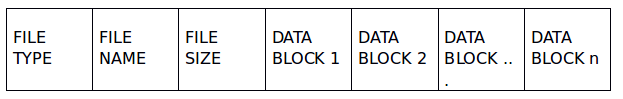
\includegraphics[scale=0.50]{Inode_table.png}
\caption{\footnotesize Structure of the Inode Table}
\label{fig_1}
\end{figure}
\subsubsection{Disk Free List}
For each block in the disk there is an entry in the Disk Free List which contains a value of either 0 or 1 indicating whether the corresponding block in the disk is free or used, respectively.
\subsection{Memory Data Structures}
\subsubsection{Process Table}
 The Process Table contains an entry for each process.  Each entry contains several fields that stores all the information pertaining to a single process and the maximum number of entries is equal to maximum number of processes allowed to exist at a single point of time in eXpOS.
\begin{figure}[ht]
\centering
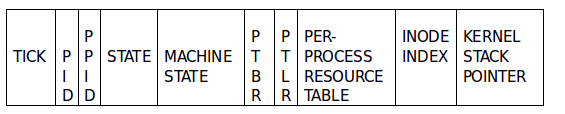
\includegraphics[scale=0.50]{Process_table.png}
\caption{\footnotesize Structure of the Process Table}
\label{fig_1}
\end{figure}

The first entry Tick keeps track of how long the process was in memory. \\
The second column is PID or Process ID which is the unique process descriptor, a number that is unique to each process.\\ 
The third column gives the process descriptor of the parent process or the PPID.\\
Next column, State , consists of a two tuple that describes the current state of the process.\\
The fifth column is the pointer to a structure that gives the Machine State when the process was last executed.  This part is machine dependent. \\
The next two columns are regarding page table of the process. The first one (PTBR or Page Table Base Register) stores the starting address of the page table of a process while the next one (PTLR or Page Table Length Register) stores the number of entries in the page table of a process and determines the size of the virtual address space of the process.\\
The next column is a pointer to a table, the Per-Process Resource Table that contains information about the files opened by the process as well as semaphores used by the process.The index of the per-process resource table entry for each resource is known as the resource descriptor.\\
Inode Index is a reference to the Inode entry of the executable file. It could be used to access the code pages of the process.\\
Each process has its own kernel stack whose pointer is given in the Kernel Stack Pointer column. A process uses its kernel stack to save the return address when it decides to voluntarily schedule out itself out when entering a blocking system call. 
\subsubsection{File Table}
File Table has information about all the files that are currently open.  It is initialized by the OS startup code.  Initially, there are no open files.
\begin{figure}[ht]
\centering
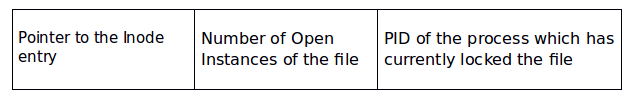
\includegraphics[scale=0.50]{File_table.png}
\caption{\footnotesize Structure of the File Table}
\label{fig_1}
\end{figure}
\subsubsection{Semaphore Table}
Semaphore Table contains details about all the semaphores used by the processes. For every semaphore opened by a process, there is an entry in the per-process resource table (which is discussed later),  and this entry points to a corresponding entry in the semaphore table.
\begin{figure}[ht]
\centering
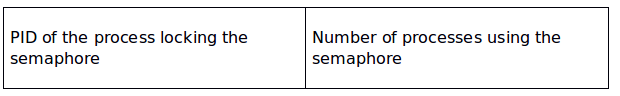
\includegraphics[scale=0.50]{Semaphore_Table.png}
\caption{\footnotesize Structure of the Semaphore Table}
\label{fig_1}
\end{figure}
\subsubsection{Disk Status Table}
eXpOS makes use of Disk Status Table to keep track of load and store operations. It consists of four entries which is given in Figure 4.
\begin{figure}[ht]
\centering
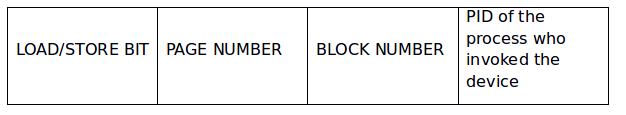
\includegraphics[scale=0.50]{Disk_Status.png}
\caption{\footnotesize Structure of the Disk Status Table}
\label{fig_1}
\end{figure}
\\ \\
\subsubsection{Buffer Table}
To minimize the number of load and store operations, eXpOS provides a buffer cache in memory which would temporarily store disk blocks. Each disk block is mapped to a unique buffer. The disk blocks will be stored back to the disk when some other blocks replace it. Only modified blocks are written back to disk.
Buffer Table keeps the information about disk blocks present in the buffer.
\begin{figure}[ht]
\centering
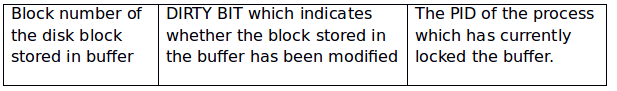
\includegraphics[scale=0.50]{Buffer_table.png}
\caption{\footnotesize Structure of the Buffer Table}
\label{fig_1}
\end{figure}
\subsubsection{System Status Table}
System Status Table keeps the information about number of free pages in memory (Mem\_free\_count), number of processes waiting for memory pages (Wait\_mem\_count) , and also the number of processes in swapped state (Swapped\_count).
\subsubsection{Memory Free List}
The Memory free list is a data structure used for keeping track of used and unused pages in the memory. Each entry of the free list contains a value of either 0 indicating whether the corresponding page in the memory is free or number indicating the number of processes that share the page.
\subsection{Algorithms}
\subsubsection{File System Calls}
%%%%% Create System Call %%%%%%%%%%%%%%%
\textbf{Create System Call}\\
The Create operation takes as input a filename and creates an empty file by that name. It also creates the root entry for the file and makes sure that every file has a unique name. Note that the file name must be a character string and must not be named “root”.
\begin{description}
\item[Arguments]: Filename
\item[Return Value]: 0 (Success) or -1 (No Space for file)
\end{description}
\begin{algorithm}
\caption{Create system call}
\begin{algorithmic}
\IF{file is present in Inode Table}
    \RETURN 0 
\ENDIF    
\IF{no free entry in Inode Table}
    \RETURN -1 
\ELSE
    \STATE store index of free entry in InodeIndex
\ENDIF   
\STATE In the Inode Table entry corresponding to InodeIndex, set file name to Filename, file size to 0 and file type to “DATA ”.
\STATE In the root file entry corresponding to InodeIndex, set file name to Filename, file size to 0 and file type to “DATA ”.
\RETURN 0 
\end{algorithmic}
\end{algorithm}
\textbf{Delete System Call}\\
Delete removes the file from the file system and removes its root entry. A file that is currently opened by any application cannot be deleted. Root file also cannot be deleted.
\begin{description}
	\item[Arguments]: Filename
	\item[Return Value]: 0 (Success) or -1 (File not found) or -2 (File is open)
\end{description} 
\begin{algorithm}
\caption{Delete system call}
\begin{algorithmic}
\IF{file is not present in Inode table}
    \RETURN -1
\ELSE
    \STATE store index of file in InodeIndex
\ENDIF    
\IF{file is open}
    \RETURN -2
\ENDIF
\STATE Free all the blocks allocated to the file
\STATE Invalidate the Inode Table entry corresponding to Inodeindex
\STATE Remove root file entry corresponding to Inodeindex
\RETURN 0 
\end{algorithmic}
\end{algorithm}
\textbf{Open System Call}\\
 For a process to read/write a file, it must first open the file. Only data and root files can be opened. The Open operation returns a file descriptor. The file descriptor conceptually refers to the location of the file which will be referred to by other file operations. The file pointer initially points to the first word in the file when Open system call is completed. An application can open the same file several times and each time a different descriptor will be returned by the Open operation. 
\begin{description}
	\item[Arguments]: Filename
	\item[Return Value]: File Descriptor (Success) or -1 (File not found) or -2 (Process has reached its limit of resources) or -3 ( 	System has reached its limit of open files)
\end{description} 
\begin{algorithm}
\caption{Open system call}
\begin{algorithmic}
\IF{file is not found in Inode Table}
    \RETURN -1
\ENDIF
\IF{file type is not DATA or ROOT}
    \RETURN -1
\ENDIF
\IF{no free entry in Per-Process Resource table}
    \RETURN -2
\ELSE
    \STATE store index of free entry in \textit{PerProcessIndex}
\ENDIF    
\IF{file is already open}
    \STATE store index of file table entry in \textit{FTIndex}
\ELSE
    \IF{no free entry in FT}
        \RETURN -2
    \ELSE 
        \STATE store index of free entry in \textit{FTIndex}
    \ENDIF
\ENDIF
\STATE In entry corresponding to \textit{PerProcessIndex}, set pointer to FT as \textit{FTIndex} and LSEEK as 0
\STATE In entry corresponding to \textit{FTIndex}, set pointer to Inode Table as \textit{InodeIndex} 
\STATE Increment file open count, set lock status to free
\RETURN \textit{PerProcessIndex} 
\end{algorithmic}
\end{algorithm}
\textbf{Close System Call}\\
After all the operations are done, the user closes the file using Close system call. 
\begin{description}
	\item[Arguments]: File Descriptor
	\item[Return Value]: 0 (Success) or -1 (File Descriptor is invalid)
\end{description} 
\begin{algorithm}
\caption{Close system call}
\begin{algorithmic}
\IF{File Descriptor is not valid}
    \RETURN -1
\ENDIF
\IF{entry in Per-Process Resource table is not valid}
    \RETURN -1
\ELSE 
    \STATE store the pointer to FIle Table in  \textit{FTIndex}
\ENDIF
\STATE Decrement file open count
\IF{file is locked by current process}
    \STATE unlock the file
\ENDIF
\IF{file open count becomes zero }
    \STATE Invalidate the File Table entry
    \ENDIF
\STATE Invalidate Per\-Process Table entry 
\RETURN 0
\end{algorithmic}
\end{algorithm}
\textbf{Read System Call}\\
Read reads one word into a string/integer variable from the position pointed by file pointer in the file specified by the input file descriptor. After each read is performed, the file pointer advances to the next word in the file. 
\begin{description}
	\item[Arguments]: File Descriptor and a Buffer to which the word is read
	\item[Return Value]: 0 (Success) or -1 (File Descriptor is invalid) or -2 (File pointer has reached the end of file)
\end{description} 
\begin{algorithm}
\caption{Read system call}
\begin{algorithmic}
\IF{File Descriptor is not valid}
    \RETURN -1
\ENDIF
\IF{entry in Per-Process Resource table is not valid}
    \RETURN -1
\ELSE 
    \STATE store the pointer to FIle Table in  \textit{FTIndex}
    \STATE store LSEEK in  \textit{lseek}
\ENDIF
\WHILE{file is locked}
    \STATE put the current process to sleep
    \STATE call scheduler
\ENDWHILE
\STATE lock the file
\STATE store pointer to Inode Table in  \textit{InodeIndex}
\IF{file pointer is at the end of the file}
    \RETURN -2
\ELSE 
    \STATE store \textit{lseek}/XFS\_MAXBSIZE in \textit{BlockNum}
    \STATE store \textit{lseek}\%XFS\_MAXBSIZE in \textit{Offset}
\ENDIF
\STATE find the buffer to which the block is mapped
\IF{buffer is locked}
    \IF{current process has not locked the buffer}
        \WHILE{buffer is locked}
            \STATE put the process to sleep
            \STATE call scheduler
        \ENDWHILE
        \STATE lock the buffer
    \ENDIF
\ELSE
    \STATE lock the buffer
\ENDIF
\IF{buffer does not have required block}
    \IF{buffer contains a block and dirty bit is set}
        \STATE store the block in buffer to disk
    \ENDIF
    \STATE load the required block to the buffer
\ENDIF
\STATE Read the data
\STATE Increment the file pointer
\STATE unlock the buffer and wake all processes waiting for the buffer
\STATE Unlock the file and wake all processes waiting for the file
\RETURN 0
\end{algorithmic}
\end{algorithm}
\textbf{Write System Call}\\
Write writes one word from a string/integer variable provided by the user, to the position pointed by input file pointer. After each write is performed, the file pointer advances to the next word in the file.
\begin{description}
	\item[Arguments]:File Descriptor and a Word to be written
	\item[Return Value]: 0 (Success) or -1 (File Descriptor given is invalid) or -2 (No disk space)
\end{description} 
\begin{algorithm}
\caption{Write system call}
\begin{algorithmic}
\IF{File Descriptor is not valid}
    \RETURN -1
\ENDIF
\IF{entry in Per-Process Resource table is not valid}
    \RETURN -1
\ELSE 
    \STATE store the pointer to FIle Table in  \textit{FTIndex} and LSEEK in  \textit{lseek}
\ENDIF
\WHILE{file is locked}
    \STATE put the current process to sleep and call scheduler
\ENDWHILE
\STATE lock the file
\STATE store pointer to Inode Table in  \textit{InodeIndex}
\STATE store \textit{lseek}/XFS\_MAXBSIZE in \textit{BlockNum} and \textit{lseek}\%XFS\_MAXBSIZE in \textit{Offset}
\IF{entry corresponding to \textit{BlockNum} is invalid}
    \IF{no free block in disk}
        \RETURN -2
    \ELSE
        \STATE allocate a free block to the file
        \STATE increment file size in Inode Table and root file
    \ENDIF
\ENDIF
\STATE find the buffer to which the block is mapped
\IF{buffer is locked}
    \IF{current process has not locked the buffer}
        \WHILE{buffer is locked}
            \STATE put the process to sleep
            \STATE call scheduler
        \ENDWHILE
        \STATE lock the buffer
    \ENDIF
\ENDIF
\STATE lock the buffer
\IF{buffer does not have required block}
    \IF{buffer contains a block and dirty bit is set}
        \STATE store the block in buffer to disk
    \ENDIF
    \STATE load the required block to the buffer
\ENDIF
\STATE Write the data 
\STATE unlock the buffer and wake all processes waiting for the buffer
\STATE Unlock the file and wake all processes waiting for the file
\RETURN 0
\end{algorithmic}
\end{algorithm}
\textbf{Seek System Call}\\
If user wants to change the file pointer without reading/writing, Seek system call is used. The Seek operation allows the application program to change the location pointed to by the file pointer from the current position to a different position in the file so that next Read/Write is performed from the new position. An Offset of 0 will reset the pointer to the start of the file. A negative Offset will move the pointer backwards.
\begin{description}
	\item[Arguments]: File Descriptor and Offset
	\item[Return Value]: 0 (Success) or -1 (File Descriptor given is invalid) or -2 (Offset value moves the file pointer to a position outside the file)
\end{description} 
\begin{algorithm}
\caption{Seek system call}
\begin{algorithmic}
\IF{File Descriptor is not valid}
    \RETURN -1
\ENDIF
\IF{entry in Per-Process Resource table is not valid}
    \RETURN -1
\ELSE 
    \STATE store the pointer to FIle Table in  \textit{FTIndex}
    \STATE store LSEEK in  \textit{lseek}
\ENDIF
\WHILE{file is locked}
    \STATE put the current process to sleep
    \STATE call scheduler
\ENDWHILE
\STATE lock the file
\STATE store pointer to Inode Table in  \textit{InodeIndex}
\IF{new file pointer is not valid}
    \RETURN -2
\ENDIF
\IF{Offset is zero}
    \STATE set LSEEK to beginning of file
\ELSE
    \STATE set LSEEK to LSEEK$+$Offset
\ENDIF
\STATE Unlock the file and wake all processes waiting for the file
\RETURN 0
\end{algorithmic}
\end{algorithm}
\subsubsection{Process System Calls}
\textbf{Fork System Call}\\
Replicates the process invoking the system call. The heap, code and library regions of the parent are shared by the child. A new stack is allocated to the child and the data in the parent stack is copied into the child stack.
\\
When a process executes the Fork system call, the child process shares with the parent all the file handles and semaphores previously opened by the parent. Note that semaphores and the files handles acquired subsequent to the fork operation by either the child or the parent will be exclusive to the respective process and will not be shared.
\begin{description}
\item[Arguments]: None
\item[Return Value]: Process Identifier to the parent process and 0 to child process (Success) or -1 (Number of processes has reached its maximum)
\end{description} 
\begin{algorithm}
\caption{Fork system call}
\begin{algorithmic}
\IF{no free entry in process table}
    \RETURN -1
\ELSE
    \STATE store index of free entry in \textit{ChildPID}
    \STATE store pid of parent process in \textit{ParentPID}
\ENDIF
\STATE set the PPID field of child process to \textit{ParentPID}
\STATE count the number of stack pages of parent
\WHILE{equal number of free pages are not present in memory}
    \STATE put the process to sleep
    \STATE call scheduler
\ENDWHILE
\STATE Allocate free pages to the child
\STATE Copy the parent's stack to child's stack
\STATE Copy the page table entries of parent, except stack entries, to the page table of child
\STATE Copy the machine state and per\-process resource table to child
\STATE For every open file of the parent, increment the file opern count
\STATE For every semaphore acquired by the parent, increment process count
\STATE set state of child to ready
\RETURN 0 to the child process and \textit{ChildPID} to the parent process
\end{algorithmic}
\end{algorithm}
\textbf{Exec System Call}\\
Exec loads the executable program into the memory address space of the calling process, overlaying the calling application with the newly loaded program. After the Fork system call, if either the parent or the child process loads another program into its virtual address space using the exec system call, then the shared heap is detached from that process and the surviving process will have the heap intact. A successful Exec operation results in extinction of the calling application and never returns to the caller application. For the new process, no heap pages are allocated. All open instances of file and semaphores of parent process is closed. 
\begin{description}
\item[Arguments]: Filename
\item[Return Value]: -1 (File not found or file is of invalid type)
\end{description} 
\begin{algorithm}
\caption{Exec system call}
\begin{algorithmic}
\IF{file not found in Inode Table}
    \RETURN -1
\ELSE
    \IF{file type is not EXEC}
        \RETURN -1
    \ELSE
        \STATE store index of Inode Table entry in \textit{InodeIndex}
        \STATE store the ode block numbers of the file in \textit{Block1} and \textit{Block2}.
    \ENDIF
\ENDIF
\STATE In the page table of current process, set code page entries to \textit{Block1} and \textit{Block2}.
\STATE Include the page numbers of shared library in the page table.
\STATE Set the auxillary information to invalid and unreferenced.
\STATE Invalidate the entry for heap pages
\STATE Close all files opened by the current process
\STATE Release all semaphores held by the parent process.
\STATE Set SP and IP values to valid locations.
\RETURN 0 
\end{algorithmic}
\end{algorithm}
\textbf{Exit System Call}\\
 Exit system call terminates the execution of the process which invoked it and removes it from the memory. It schedules the next ready process and starts executing it. When there is no other ready process to run, it halts the machine.
\begin{description}
\item[Arguments]: None
\item[Return Value]: -1 (Failure)
\end{description} 
\begin{algorithm}
\caption{Exit system call}
\begin{algorithmic}
\IF{no more processes to schedule}
    \STATE shutdown the machine
\ELSE 
    \STATE store the pid of the next ready process in \textit{NextPID}
\ENDIF
\STATE Close all files opened by the current process
\STATE Release all the semaphores used by the current process
\STATE Memory pages of the current process are freed
\STATE Invalidate the page table entry
\STATE Wake up all processes waiting for the current process
\STATE Schedule the process with pid \textit{NextPID}
\RETURN 
\end{algorithmic}
\end{algorithm}
\textbf{Getpid System Call}\\
 Returns the process identifier of the invoking process.
\begin{description}
\item[Arguments]: None
\item[Return Value]: Process Identifier (Success) or -1 (Failure)
\end{description} 
\begin{algorithm}
\caption{Getpid system call}
\begin{algorithmic}
\STATE Find the PID of the current process by using PTBR value.
\RETURN PID of current process
\end{algorithmic}
\end{algorithm}
\textbf{Getppid System Call}\\
Returns the process Identifier of the parent of the invoking process.
\begin{description}
\item[Arguments]: None
\item[Return Value]: Process Identifier (Success) or -1 (Failure)
\end{description} 
\begin{algorithm}
\caption{Getppid system call}
\begin{algorithmic}
\STATE Find the PID of the current process by using PTBR value.
\STATE From the Process Table entry of the current process, find the PPID
\RETURN PPID of current process
\end{algorithmic}
\end{algorithm}
\textbf{Shutdown System Call}
Shutdown system call terminates all processes, writes modified(dirty) pages and memory copy of disk data structures to the disk, and then halts the machine. In case the system call failed, an error is returned to the invoking process. 
\begin{description}
\item[Arguments]: None
\item[Return Value]: -1 (failure)
\end{description} 
\begin{algorithm}
\caption{Shutdown system call}
\begin{algorithmic}
\WHILE{disk is not free}
    \STATE put the process to sleep
    \STATE call scheduler
\ENDWHILE
\STATE store Inode Table to the disk
\STATE store dirty pages to disk
\STATE store Disk Free List to the disk
\STATE Halt the machine
\RETURN 
\end{algorithmic}
\end{algorithm}
\section{Work Done}
\begin {itemize}
\item The existing OS data structures were redesigned to incorporate the changes done. 
\item New data structures like Buffer Table, Disk Status Table, Semaphore Table etc were designed.
\item System calls were redesigned to incorporate asynchronous operations, buffer cache and pre-emptive scheduling.
\item Directory structure was introduced in eXpFS.
\item Executable file format was designed.
\end{itemize}
 
\section{Future Work}
Future work includes implementation of all the features mentioned above, testing of the system and building a roadmap for anyone wishing to build eXpOS.
\section{Conclusion}
This project aims to create a simpler version of an operating system which allows students to acquire insight into the working of a real operating system. 

\begin{thebibliography}{1}
\bibitem{latexMath}\texttt{$http://xosnitc.github.io/$}
\bibitem {2} The Design of Unix Operating System, By Maurice J. Bach
\end{thebibliography}

\end{document}
